% Author :  Lionel du Peloux
% Contact : lionel.dupeloux@gmail
% Year : 2017
% !TEX encoding = UTF-8 Unicode

\chapter{Elastic rod~: variational approach}
\label{sec:ch_energy}

This chapter should be understood as an extension of the work initiated by \citef{Tayeb2015a} and published by \citef{DuPeloux2015} and \citef{Lefevre2017}.

% #######################################################
\section{Introduction}
% #######################################################

Elastic gridshells are lightweight structures made of interconnected slender beams (see \cref{chp:gridshell}). Modeling the deformation process of such structures is complex as it involves to take account for the geometric non linearities induced by the large displacements and rotations of the grid. More over, the large number of connexions and the coupling between flexion and torsion highly increase the complexity of the analysis.

To facilitate the design process of elastic gridshells, architects and engineers need a dedicated numerical tool that provide a good level of interactivity -- which means that numerical computations must converge within a reasonable time, if not in real time -- and gives deep insights on the geometry and on the mechanical behavior of the grid. This tool must be able to model complex connexions and various types of support conditions to enhance the user experience during the formfinding stage and to improve his ability to explore the space of constructible shapes.

In this chapter, our goal is to develop a beam model suitable for the modeling of grids of interconnected slender beams in order to study the mechanics of elastic gridshells. For such beams, Kirchhoff's theory of rods is considered to be appropriate. We follow recent advances in the field of computer graphics about hair modeling \cite{Bergou2008} to build a reduced degrees of freedom rod model thanks to an appropriate curve-angle representation. This representation is based on a relevant curve framing, namely the Bishop frame presented in \cref{sec:bishop}. The rod will be considered inextensible. Moreover, it will be assumed that cross-sections remain normal to the rod centerline. The internal forces and moments acting on the rod will be deduced from the differentiation of the elastic energy of the beam with respect to the degrees of freedom of the system.

This chapter is devoted to the development of the beam model. The formulation of a discrete element and its implementation in a numerical solver are treated in a dedicated chapter (see \cref{chp:numerical_model}).

\subsection{Overview}
We begin this chapter by establishing a representation for any geometric configuration of a Kirchhoff rod (see \cref{sec:kirchhoff_rod}) based on a curve-angle description. This representation is 

\subsection{Contributions}
\begin{itemize}
\item We consolidate the mathematical development of the beam model by introducing the Fréchet and Gateaux derivatives in function spaces.
\item We clarify the independence of the the rotational degree of freedom ($\theta$) with respect to  translational degrees of freedom ($\vect{x}$).
\item We factorize the expressions of the internal forces and moments by reusing the quasi-static assumption.
\item We identify the contributions of axial and shear forces, bending and torsion moments in the expressions of internal forces and moments.
\item We prove the equivalence with the shear force obtained from the dynamical equations of Kirchhoff.
\item We suggest that the dynamical Kirchhoff equations should be a more straight forward starting point to build up similar theories.
\end{itemize}

\subsection{Related work}
\citef{Bergou2008} present a discrete treatment of adapted framed curves, parallel transport, and holonomy. Based on this framework they propose a curve-angle representation of the geometric configuration of slender rods. In this representation, the orientation of the material frame is established with respect to the Bishop frame by a single scalar angle. Upon this representation they build a mechanical model for slender elastic rods with anisotropic cross-section and arbitrary rest configuration. In the dynamic the centerline is treated explicitly and material frames are treated as quasistatic. \citef{Bergou2010} improve there previous model for the modeling of viscous threads.

\citef{Nabaei2014} implements the model developed by \cite{Bergou2008} in IPOPT, an interior point optimizer, to solve the static equilibrium of simply connected systems of twisted elastica.

\citef{Tayeb2015a}, \citef{DuPeloux2015} and \citef{Lefevre2017} follow \cite{Bergou2008} to model grids of interconnected slender beams. They implement their model in a dynamic relaxation solver to formfind elastic gridshells. They formulate a special connexion.

\cite{Spillmann2007}.
\cite{Fuller1978},~\cite{deVries2005}, ~\cite{Vauquelin2000},~\cite{Berger2009}

Bertail
Spilmann
Hose
Pour intro~:~\cite{Jung2010}






%\note{
%\begin{enumerate}
%\item quaternion pour piloter les input / ouput ?
%\item calcul de la hessienne au moins pour les $\theta$ comme Audoly. Ne serait-ce pas possible pour les $x$ ?  Avec ma technique du transport parallèle il me semble pourvoir avoir accès au DL à  l'ordre 2 \dots
%\item Formulation pour les efforts ponctuels / moments extérieurs en vue d'une résolution par minimisation. Voir F. Bertails
%\item prise en compte des contraintes => méméthide des multiplicateurs de lagrange
%\end{enumerate}
%}

% #######################################################
\section{Kirchhoff rod}\label{sec:kirchhoff_rod}
Kirchhoff's theory of rods is presented thoroughly in the next chapter (see \cref{chp:kirchhoff}). In this chapter, although the assumptions are not exactly the ones made by  Kirchhoff in his theory, we will stick to this denomination as introduced by \cite{Bergou2008}. In the present theory we will assume that~:
\begin{itemize}
\item the rod is inextensible,
\item cross-sections remain plane,
\item cross-sections remain perpendicular to the centerline,
\item the material deforms elastically.
\end{itemize}

\subsection{Description of the motion}\label{sec:description_motion}
We introduce a curvilinear coordinate system to describe the motion of our Kirchhoff rod. It is composed of a parametric space curve, called the \emph{centerline}, equipped with a moving frame, called the \emph{material frame}.

\subsubsection{Deformed configuration}
The actual geometric configuration of the rod is described by its centerline $\vect{x}(s)$ and its cross-sections. The centerline is a space curve parameterized by its arc length, denoted $s$. Cross-sections orientation are followed along the centerline by a material frame $\{\vect{d}_3 (s),\vect{d}_1 (s),\vect{d}_2 (s)\}$ which is an adapted orthonormal moving frame aligned with the principal axes of inertia of the cross-section.

Recall from \cref{sec:amf} that \emph{adapted} means that the material frame is aligned with the tangent vector of the centerline~:
\begin{equation}
	\vect{d}_3 (s)=\vect{x}'(s)=\vect{t}(s)
\end{equation}
Here, the prime symbol denotes the derivation with respect to the arc length parameter $s$. Recall also from \cref{sec:arclength_param} that $\norm{\vect{x}'(s)}=1$ because $\vect{x}$ is parametrized by arc length.

\subsubsection{Stress-free configuration}
Among all the possible geometric configurations of the rod we identify the \emph{stress-free configuration} or \emph{rest configuration}, that is the configuration in which the rod is stress-free under no external forces and moments applied top it (loads, supports, \telp{}). This configuration is crucial as the elastic energy of a rod in a given configuration relies on both its actual and rest configuration.

Hereinafter, the symbols referring to this configuration will be denoted with an overbar (e.g. $\overbar{\vect{x}}(s)$).

\subsection{Inextensibility assumption}
As explained by \citef{Audoly2010}, based on a scaling argument, two cases arise for slender beams~: either the centerline stretches and bending and twisting forces become negligible compared to axial forces~; either the centerline remains inextensible. As we are not interested in the first case -- in which the beam would behave like a cable, mainly in tension -- we will assume that the rod is effectively inextensible.\footnote{For a complete treatment of the question of inextensibility refer to \cref{sec:kirchhoff_motion} in \cref{chp:kirchhoff}.}

Remark that the previous description (see \cref{sec:description_motion}) is only valid for inextensible rods. Indeed, for an inextensible rod the centerline does not stretches and the arc length parameter for the rest configuration is also a valid arc length parameter for any other configuration.\footnote{For a complete treatment of the question of reparametrization refer to \cref{sec:cosserat_motion} in \cref{chp:kirchhoff}.}

Hereinafter, the length of the rod will be denoted $L$ and the arc length $s$ will vary in $[0,L]$, with no loss of generality.

\subsection{Euler-Bernouilli assumption}
Strains are supposed to remain small so that the cross-sections remain plane and the material frame remain orthonormal and adapted to the centerline during the motion of the rod. In other words the cross-sections undergo rigid body motions.\footnote{For a complete treatment of this point in Kirchhoff's theory refer to \cref{sec:kirchhoff_deform_conf} in \cref{chp:kirchhoff}.}

\subsection{Governing equations}
Thus, differentiating the conditions of orthonormality of the material frame (see \cref{sec:moving_frame}) leads to the following system of differential equations governing the evolution of the \emph{material directors} $\{\vect{d}_3 (s),\vect{d}_1 (s),\vect{d}_2 (s)\}$ along the centerline~:
\begin{equation} \label{eq:3_1}
	\begin{bmatrix}
		\vect{d}'_3(s) \\
		\vect{d}'_1(s) \\
		\vect{d}'_2(s)
	\end{bmatrix}
	=
	\begin{bmatrix}
		0 & \kappa_{2}(s) & -\kappa_{1}(s) \\
		-\kappa_{2}(s) & 0 & \tau(s) \\
		\kappa_{1}(s) & -\tau(s) & 0
	\end{bmatrix}
	\begin{bmatrix}
		\vect{d}_3(s) \\
		\vect{d}_1(s) \\
		\vect{d}_2(s)
	\end{bmatrix}
\end{equation}
These equations can be formulated with the \emph{Darboux vector} of the chosen material frame, which represents the angular velocity vector of the frame along $\vect{x}(s)$~:
\begin{subequations}
	\begin{alignat}{2}
		&\vect{d}'_{i}(s) = \vect{\Omega}_m(s) \times \vect{d}_i(s)
		\\[0.5em]
		&\vect{\Omega}_m(s) = \begin{bmatrix} \tau(s) \\ \kappa_{1}(s) \\ \kappa_{2}(s)
	\end{bmatrix}
	\end{alignat}
\end{subequations}

where $\tau(s)$, $\kappa_{1}(s)$ and $\kappa_{2}(s)$ represent the components of the angular velocity of the material frame around its axes $\vect{d}_3 (s)$, $\vect{d}_1 (s)$ and $\vect{d}_2 (s)$ when it travels along the centerline at unit speed.\footnote{See \cref{fig:geo_interpretation} in \cref{sec:moving_frame} for a geometric interpretation of these rates of rotation.}

\subsection{Curvatures and twist}
The material curvatures are denoted $\kappa_1(s)$ and $\kappa_2(s)$ and represent the rod's flexion in the principal planes respectively normal to $\vect{d}_1(s)$ and $\vect{d}_2(s)$.The material twist is denoted $\tau(s)$ and represents the section's rate of rotation around $\vect{d}_3(s)$. Those scalar functions measure directly the strain as defined in Kirchhoff's theory.\footnote{For a complete treatment of the definition of material strains refer to \cref{sec:kirchhoff_strains} in \cref{chp:kirchhoff}.}

Recall from \cref{sec:curvature} that the Frenet frame $\{\vect{t}(s),\vect{n}(s),\vect{b}(s)\}$ defines the osculating plane and the curvature ($\kappa$) of a spatial curve~:
\begin{subequations}
	\begin{alignat}{2}
		&\vect{t}'(s) = \vect{x}''(s) = \kappa(s) \cdot \vect{n}(s)
		\\
		&\kappa(s) = \norm{\vect{t}'(s)} = \norm{\vect{x}''(s)}
		\\
		&\vect{b}(s) = \vect{t}(s) \times \vect{n}(s)
	\end{alignat}
\end{subequations}
To describe the osculating plane in which lies the bending part of the deformation we rely on the \emph{curvature binormal} introduced previously in \cref{eq:kb}~:
\begin{equation}
	\vect{\kappa b}(s) = \vect{t}(s)\times\vect{t}'(s) = \kappa(s) \cdot \vect{b}(s)
\end{equation}
The curvature binormal is the vector of direction $\vect{b}(s)$ and norm $\kappa(s)$. At each point of arc length $s$ the osculating plane is normal to $\vect{\kappa b}(s)$.

\subsection{Elastic energy}
Kirchhoff's theory assigns an elastic energy to beams according to their strain~\cite{Audoly2010}. In this theory, a beam is supposed to be inextensible. Thus the elastic energy ($\mathcal{E}$) only accounts for torsion and bending behaviors and is given by~:
\begin{equation}
	\mathcal{E} =
	\tfrac{1}{2} \int_{0}^{L}EI_1(\kappa_1-\rconf{\kappa}_1)^2 + EI_2(\kappa_2-\rconf{\kappa}_2)^2 ds
	+ \tfrac{1}{2} \int_{0}^{L} GJ(\tau -{\rconf{\tau}})^2 ds
\end{equation}
Here, $\rconf{\kappa}_1$, $\rconf{\kappa}_2$ and $\rconf{\tau}$  denote the natural material curvatures and material twist of the rod in the rest configuration. $E$ and $G$ are the elastic and shear modulus of the material. $I_1$ and $I_2$ are the moments of inertia of the cross-section. $J$ is the torsion constant of the cross-section.

\section{Curve-angle representation}

In the previous paragraph we have shown how the elastic energy of a rod can be computed with respect to the position of its centerline and the orientation of its cross-sections. This representation can be naturally described with six degrees of freedom (\dofs{6})~:\footnote{This is the usual choice where the orientation of the material frame is parametrized by a rotation matrix, or equivalently a quaternion.}
\begin{itemize}
\item \dofs{3} for the position of the centerline,
\item and \dofs{3} for the orientation of the cross-sections.
\end{itemize}

Following~\citef{Bergou2008} we introduce a reduced coordinate formulation of the rod that accounts for only \dofs{4}~:
\begin{itemize}
\item \dofs{3} for the position of the centerline,
\item and only \dofs{1} for the orientation of the cross-sections.
\end{itemize}
This reduction of the number of \dofs{} relies on the choice of a suitable reference frame, namely a Bishop (or zero-twisting) frame denoted $\{\vect{t}(s),\vect{u}(s),\vect{v}(s)\}$. Recall fom \cref{sec:bishop} in \cref{chp:curve} that this reference frame is adapted to the centerline and exhibits a null angular velocity around the centerline's tangent vector, which means~:
\begin{equation}
	\vect{u}\cdot\vect{v}' = \vect{u'}\cdot\vect{v}=0
\end{equation}
The Bishop frame only depends on $\vect{x}$, the geometry of the centerline, depending on the choice of an initial condition. This reference frame is obtained alla along the curve by propagating a given initial frame (at $s=0$) with parallel transport (see \cref{sec:paralleltransport}). By construction, this reference frame evolves along the curve at angular velocity~:
\begin{equation}
	\vect{\Omega}_b(s)=\vect{\kappa b}=\vect{t}\times\vect{t'}
\end{equation}
Remark that $\vect{\Omega}_b(s)$ only depends on the centerline and is well defined even when the curvature vanishes (whereas the Frenet frame would be undefined when the curvature vanishes). In that case the parallel transport operator becomes the rotation of null angle, which is still a valid transformation.


 Thus, cross section orientations $\{\vect{d}_3 (s),\vect{d}_1 (s),\vect{d}_2 (s)\}$ can be tracked only by the measure of an angle $\theta$ from this reference frame denoted $\{\vect{d}_3(s),\vect{u}(s),\vect{v}(s)\}$ (Figure 5).

Note that an alternative solution could be to parameterize the global rotations of local material frame and to compute the rotation needed to align two successive frames along the curve's tangent.

\note{
Ici, expliquer la succession des dépendances~: les vecteurs matériaux dépendent du repère de bishop par la seule variable theta. Le repère de bishop quand à  lui est entièrement déterminé (au choix d'une constante de départ près) par la donnée de la centerline x.

Faire un schéma explicatif.

quid du transport parallèle en temps et non en espace ?
}

\begin{figure}[t]
%	\begin{fullpage}
		\captionsetup[subfloat]{captionskip=10pt}
     		\centering
     		\subfloat[][succession of degrees of freedom]{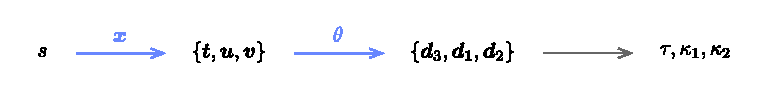
\includegraphics{degrees_of_freedom.pdf}\label{fig:curve_angle_a}}
		\vspace{10pt}
		%
		\subfloat[][bending strains]{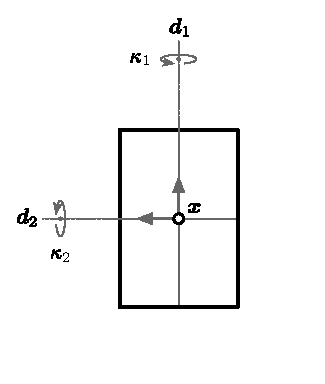
\includegraphics{curve_angle_a.pdf}\label{fig:curve_angle_b}}
		\hspace{2.5cm}
		\subfloat[][angular deviation]{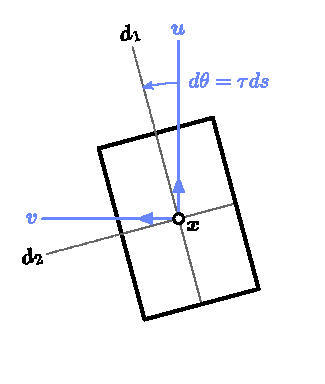
\includegraphics{curve_angle_b.pdf}\label{fig:curve_angle_c}} \\
		\vspace{20pt}
		%
		\caption[Curve-angle representation of the rod]{Curve-angle representation of the rod. The orientation of the material frame is established from the reference frame by its angular deviation $\theta(s)$.}
		\label{fig:curve_angle}    
%	\end{fullpage}
\end{figure}

\subsection{Zero-twisting frame}
Zero-twisting frame, also known as Bishop frame, was introduced by Bishop in 1964. Bishop remarked that there was more than one way to frame a curve~\cite{Bishop1975}. Indeed, for a given curve, any orthonormal moving frame would satisfy the following differential equations, where $k_1(s)$, $k_2 (s)$ and $\tau(s)$ are scalar functions that define completely the moving frame~:
\begin{gather}
	\begin{bmatrix}
		\mathbf{e'_{3}}(s) \\
		\mathbf{e'_{1}}(s) \\
		\mathbf{e'_{2}}(s)
	\end{bmatrix}
=
	\begin{bmatrix}
		0 & k_{2}(s) & -k_{1}(s) \\
		-k_{2}(s) & 0 & \tau(s) \\
		k_{1}(s) & -\tau(s) & 0
	\end{bmatrix}
	\begin{bmatrix}
		\mathbf{e_{3}}(s) \\
		\mathbf{e_{1}}(s) \\
		\mathbf{e_{2}}(s)
	\end{bmatrix}
\end{gather}
For instance, a Frenet frame $\{\vect{t}(s),\vect{n}(s),\vect{b}(s)\}$ is a frame which satisfies $k_1(s)=0$. Note that this frame suffers from major disadvantages~: it is undefined where the curvature vanishes and it flips at inflexion points.
A Bishop frame $\{\vect{t}(s),\vect{u}(s),\vect{v}(s)\}$ is a frame which satisfies $\tau(s)=0$. By construction, this frame has no angular velocity (i.e. no twist) around the curve's tangent ($\vect{u}\cdot\vect{v}' = \vect{u'}\cdot\vect{v}=0$). Its evolution along the curve is described by the corresponding Darboux vector~: $\vect{\Omega}_b(s)=\vect{\kappa b}=\vect{t}\times\vect{t'}$. 
\section{Strains}

\subsection{Axial strain}
There is no axial strain to be considered as far as the rod is supposed to be unstretchable.

Remark that the inextensibility hypothesis implies that any admissible perturbation ($\lambda\vect{h}_x$) of the rod's centerline ($\vect{x}$) is locally orthogonal to the centerline itself. Indeed, at each arc length $s$ an inextensible rod must satisfies~:
\begin{equation}\label{eq:3_6}
	\|\vect{x}'\| = \|(\vect{x}+\lambda\vect{h}_x)'\| = 1 \Rightarrow \vect{d}_3 \cdot \vect{h}'_x = -\tfrac{\lambda^2}{2}\|\vect{h}'_x\|^2 = o(\lambda) \simeq 0
\end{equation}

In other words, this means that the same arc length parametrization can be used to locate beam sections along the centerline along the deformation path. This would not be the case if the centerline would shorten or stretch out during its deformation. It is worth to mention here that this property ($\vect{d}_3 \cdot \vect{h}'_x = 0$) will be used several times in the following sections.

\subsection{Bending strain}

Let's compute the bending strains $\kappa_1$ and $\kappa_2$ regarding the geometric configuration of the rod. Remark that~:
\begin{subequations}
	\begin{gather}
	\vect{\kappa b}\cdot\vect{d}_1 = (\vect{d}_3\times\vect{d}'_3)\cdot\vect{d}_1 = (\vect{d}_1\times\vect{d}_3)\cdot\vect{d}'_3 = -\vect{d}_2\cdot\vect{d}'_3 = \kappa_1 \\
	\vect{\kappa b}\cdot\vect{d}_2 = (\vect{d}_3\times\vect{d}'_3)\cdot\vect{d}_2 = (\vect{d}_2\times\vect{d}_3)\cdot\vect{d}'_3 = \vect{d}_1\cdot\vect{d}'_3 = \kappa_2
	\end{gather}
\end{subequations}
That is to say $\vect{\kappa b}$ is orthogonal to $\vect{d}_3$~:
\begin{equation}
	\vect{\kappa b} = \kappa_1\vect{d}_1 +   \kappa_2\vect{d}_2
\end{equation}
Thus, the vector of material curvatures ($\vect{\omega}$) expressed on material frame axes $\{\vect{d}_1(s),\vect{d}_2(s)\}$ is defined as~:
\begin{equation}
	\vect{\omega} =
	\begin{bmatrix}
		\kappa_1\\
		\kappa_2\\
	\end{bmatrix} =
	\begin{bmatrix}
		\vect{\kappa b}\cdot\vect{d}_1\\
		\vect{\kappa b}\cdot\vect{d}_2\\
	\end{bmatrix} =
		\begin{bmatrix}
		-\vect{x}''\cdot\vect{d}_2\\
		\vect{x}''\cdot\vect{d}_1\\
	\end{bmatrix}
\end{equation}

\subsection{Torsional strain}
Let's compute the twist or torsional strain $\tau$ regarding the geometric configuration of the rod. Decomposing the material frame on the bishop frame gives~:
\begin{equation}
	\begin{bmatrix}
		\vect{d}_1\\
		\vect{d}_2\\
	\end{bmatrix} =
		\begin{bmatrix}
		\cos{\theta} & \sin{\theta}\\
		-\sin{\theta} & \cos{\theta}\\
	\end{bmatrix}
	\begin{bmatrix}
		\vect{u}\\
		\vect{v}\\
	\end{bmatrix}
\end{equation}
Thus, the twist can be identified directly as the variation of $\theta$ along the curve~:
\begin{equation}
	\tau = \vect{d}'_1 \cdot \vect{d}_2 = (\theta'\vect{d}_2 + \vect{\kappa b}\times\vect{d}_1)\cdot \vect{d}_2 = \theta' + \vect{d}_3\cdot\vect{\kappa b} = \theta'
\end{equation}
Note that the Frenet frame does not lead to a correct evaluation of the twist.

\section{Elastic energy}
Introducing $\vect{\omega}$ and $\theta$, the elastic energy can be rewritten as follow~:
\begin{equation}
		\mathcal{E} = \mathcal{E}_{b} + \mathcal{E}_{t} =
		\tfrac{1}{2} \int_{0}^{L} (\vect{\omega}-\rconf{\vect{\omega}})^T B (\vect{\omega}-\rconf{\vect{\omega}}) ds
		+ \tfrac{1}{2} \int_{0}^{L} \beta(\theta' -{\rconf{\theta}'})^2 ds
\end{equation}
Where $B$ is the bending stiffness matrix along the principal axes of inertia and $\beta$ is the torsional stiffness~:
\begin{equation}
	B = \begin{bmatrix}
			EI_1	&	0\\
			0	&	EI_2\\
		\end{bmatrix}
	\quad,\quad
	\beta = GJ
\end{equation}

Recall that the rod is supposed to be inextensible in Kirchhoff's theory. Thus, there is no stretching energy associated with an axial strain. However, this constraint may be enforced via a penalty energy, which in practice is somehow very similar as considering an axial stiffness into the beam's

\note{
Remark that the twisting energy ($\mathcal{E}_{t}$) only depends on $\theta$ and is independent regarding $\vect{x}$ while the bending energy ($\mathcal{E}_{b}$) depends on both $\theta$ and $\vect{x}$ variables (remind that $\kappa_1$ and $\kappa_2$ are the projections of $\vect{\kappa b}$ over $\vect{d}_1$ over $\vect{d}_2$). Thus, a coupling between bending and twisting appears as the minimum of the whole elastic energy is not necessarily reached for concomitant minimums of bending and twisting energies.

From this energy formulation, an interesting an well-known result on elastic rods could be highlighted~: \guil{torsion is uniform in an isotropic rod that is straight in its rest configuration}~\cite{Adriaenssens1999}.

Indeed, let's take an isotropic rod ($EI_1 = EI_2 = EI$) that is straight in its rest configuration ($\rconf{\kappa}_1 = \rconf{\kappa}_2 = 0$). Then, the bending energy becomes~: $\mathcal{E}_{b} = EI_1\kappa_1^2 + EI_2\kappa_2^2 = EI\kappa^2$, and consequently doesn't depends on $\theta$ anymore. The curvature of the rod only depends on the geometry of its centerline ($\kappa = ||\vect{\kappa b}|| = ||\vect{x}'\times\vect{x}''||$). Thus, there is no more coupling between bending and twisting and the global minimum of elastic energy is reached while minimizing separately bending an twisting energies. That is to say the geometry of the rod ($\vect{x}$) is the one that minimized $\mathcal{E}_{b}$. The minimum of $\mathcal{E}_{t}$ is zero and is achieved for a uniform twist along the centerline, only prescribed by the boundary conditions.}

\section{Quasistatic assumption}
Following~\cite{Bergou2008}, it is relevant to assume that the propagation of twist waves is instantaneous compared to the one of bending waves. Thus, internal forces $\vect{f}^{int}$ and moment of torsion $\vect{m}^{int}$ acts on two different timescales in the rod dynamic. Thus on the timescale of action of the force $\vect{f}^{int}$ on the center line, driving the bending waves, the twist waves propagate instantaneously, so that $\forall s \in [0,L],\; \delta\mathcal{E}/\delta\theta=0$ for the computation of $\vect{f}^{int}$. This assumption may not be enforced, as in~\cite{Nabei2014}, but leads to simpler and faster computations.

\section{Energy gradient with respect to $\theta$~: moment of torsion}
Internal moment of torsion and forces acting on the rod are classically obtained by differentiating the potential energy of the system with respect to $\theta$ and $\vect{x}$. Here, the calculus is a bit tricky as far as the differentiation takes place in function spaces. After a brief reminder on functional derivative, the main results of the calculations of the energy derivatives are given.

\subsection{Derivative of material directors with respect to $\theta$}

Recalling that $\theta$ and $\vect{x}$ are independant variables and that Bishop frame $\{\vect{u},\vect{v}\}$ only depends on $\vect{x}$, the decomposition of material frame directors $\{\vect{d}_1,\vect{d}_2\}$ on Bishop frame leads directly to the following expression for the derivative of the material directors ~:
\begin{subequations}
%	\left\{
	\begin{gather}
	\pdiffof{\theta}{\vect{d}_1}{s}{h_\theta}
	= \frac{d}{d\lambda} \vect{d}_1[\theta + \lambda h_\theta]\Bigr|_{\lambda = 0}
	= \left(-\sin{\theta}\;\vect{u} + \cos{\theta}\;\vect{v}\right) \cdot h_\theta
	= \vect{d}_2\cdot h_\theta \\
	\pdiffof{\theta}{\vect{d}_2}{s}{h_\theta}
	= \frac{d}{d\lambda} \vect{d}_2[\theta + \lambda h_\theta]\Bigr|_{\lambda = 0}
	= \left(-\cos{\theta}\;\vect{u} - \sin{\theta}\;\vect{v}\right) \cdot h_\theta
	= -\vect{d}_1\cdot h_\theta
	\end{gather}
%	\right.
\end{subequations}

\subsection{Derivative of the material curvatures vector with respect to $\theta$}
Regarding the definition of the material curvatures vector and the derivative of material directors with respect to $\theta$, it follows immediately that~:
\begin{equation}
			\pdiffof{\theta}{\vect{\omega}}{s}{h_\theta}
	= \frac{d}{d\lambda} \vect{\omega}[\theta + \lambda h_\theta]\Bigr|_{\lambda = 0}
	= \begin{bmatrix}
		\vect{\kappa b}\cdot\vect{d}_2\\
		-\vect{\kappa b}\cdot\vect{d}_1\\
	\end{bmatrix}\cdot h_\theta
	= - \mat{J}\vect{\omega}\cdot h_\theta\\
\end{equation}
Where $\mat{J}$ is the matrix that acts on
two dimensional vectors by counter-clockwise rotation of angle $\frac{\pi}{2}$~:
\begin{equation}
	\mat{J} = \begin{bmatrix}
			0	&	-1\\
			1	&	0\\
		\end{bmatrix}
\end{equation}

\subsection{Computation of the moment of torsion}

The moment of torsion is given by the functional derivative of the potential elastic energy with respect to $\theta$ which can be decomposed according to the chaine rule~:
\begin{equation}
	\begin{aligned}
	\scalar{-m(s)}{h_\theta} = \pdiffof{\theta}{\mathcal{E}}{s}{h_\theta}
	&= \pdiffof{\theta}{\mathcal{E}_b}{s}{h_\theta} + \pdiffof{\theta}{\mathcal{E}_t}{s}{h_\theta} \\
	&= \pdiffof{\theta}{\mathcal{E}_b[\vect{\omega}[\theta]]}{s}{h_\theta} + \pdiffof{\theta}{\mathcal{E}_t[\theta]}{s}{h_\theta} \\
	\end{aligned}
\end{equation}

\subsubsection{Derivative of the torsion energy with respect to $\theta$}

Decomposing the previous calculus gives:
\begin{equation}
	\begin{aligned}
	\pdiffof{\theta}{\mathcal{E}_t[\theta]}{s}{h_\theta}
		&= \frac{d}{d\lambda} \mathcal{E}_t[\theta + \lambda h_\theta]\Bigr|_{\lambda = 0} \\
		&= \frac{d}{d\lambda}\left( \tfrac{1}{2} \int_{0}^{L} \beta\left((\theta + \lambda h_\theta)' -{\rconf{\theta}'}\right)^2 \;dt \right)\Bigr|_{\lambda = 0} \\
		&= \int_{0}^{L} \beta(\theta' -{\rconf{\theta}'}) \cdot h_\theta' \;dt \\
		&= \left[\beta(\theta' -{\rconf{\theta}'}) \cdot h_\theta\right]_0^L - \int_{0}^{L} \left(\beta(\theta' -{\rconf{\theta}'})\right)' \cdot h_\theta \;dt \\
		&= \int_{0}^{L} \left(\beta(\theta' -{\rconf{\theta}'})(\delta_L-\delta_0) - \left(\beta(\theta' -{\rconf{\theta}'})\right)'\right) \cdot h_\theta \;dt \\
	\end{aligned}
\end{equation}

\subsubsection{Derivative of the bending energy with respect to $\theta$}

The derivative of $\mathcal{E}_b$ is obtained with the chaine rule~:
\begin{equation}
	\begin{aligned}
	\pdiffof{\omega}{\mathcal{E}_b[\vect{\omega}]}{s}{\vect{h}_\omega}
		&= \frac{d}{d\lambda} \mathcal{E}_b[\vect{\omega} + \lambda \vect{h}_\omega]\Bigr|_{\lambda = 0} \\
		&= \frac{d}{d\lambda}\left( \tfrac{1}{2} \int_{0}^{L} \left((\vect{\omega} + \lambda \vect{h}_\omega)-\rconf{\vect{\omega}}\right)^T \mat{B} \left((\vect{\omega} + \lambda \vect{h}_\omega)-\rconf{\vect{\omega}}\right) \;dt \right)\Bigr|_{\lambda = 0} \\
		&= \int_{0}^{L} (\vect{\omega} - \rconf{\vect{\omega}})^T \mat{B} \cdot \vect{h}_\omega \;dt \\
	\end{aligned}
\end{equation}
Finally, reminding eq 4.14~:
\begin{equation}
	\begin{aligned}
	\pdiffof{\theta}{\mathcal{E}_b[\vect{\omega}[\theta]]}{s}{h_\theta} &=
	\pdiffof{\omega}{\mathcal{E}_b[\vect{\omega}]}{s}{(\pdiffof{\theta}{\vect{\omega}[\theta]}{s}{h_\theta})} \\
	&= - \int_{0}^{L} (\vect{\omega} - \rconf{\vect{\omega}})^T \mat{B} \mat{J}\vect{\omega}\cdot h_\theta \;dt
	\end{aligned}
\end{equation}

\subsubsection{Moment of torsion}
Thus, the
\begin{equation}
	\begin{aligned}
		\scalar{-m(s)}{h_\theta} &= \pdiffof{\theta}{\mathcal{E}_b[\vect{\omega}[\theta]]}{s}{h_\theta} + \pdiffof{\theta}{\mathcal{E}_t[\theta]}{s}{h_\theta} \\
		&= \int_{0}^{L} \left(\left(\beta(\theta' -{\rconf{\theta}'})(\delta_L-\delta_0) - \left(\beta(\theta' -{\rconf{\theta}'})\right)'\right) - (\vect{\omega} - \rconf{\vect{\omega}})^T \mat{B} \mat{J}\vect{\omega}\right) \cdot h_\theta \;dt
	\end{aligned}
\end{equation}
Finally, we can conclude on the expression of the internal moment of torsion~:
\begin{equation}
	m(s) = - \left(\beta(\theta' -{\rconf{\theta}'})(\delta_L-\delta_0) - \left(\beta(\theta' -{\rconf{\theta}'})\right)'\right) + (\vect{\omega} - \rconf{\vect{\omega}})^T \mat{B} \mat{J}\vect{\omega}
\end{equation}

\subsubsection{Quasistatic hypothesis}
\begin{equation}
	\left(\beta(\theta' -{\rconf{\theta}'})\right)' + (\vect{\omega} - \rconf{\vect{\omega}})^T \mat{B} \mat{J}\vect{\omega} = 0
\end{equation}



\section{Energy gradient with respect to $x$~: internal forces}

Internal torsional moments and forces acting on the rod are classically obtained by differentiating the potential energy of the system with respect to $\theta$ and $\vect{x}$. Here, the calculus is a bit tricky as far as the differentiation takes place in function spaces. After a brief reminder on functional derivative, the main results of the calculations of the energy derivatives are given.

\note{paragraphe entièrment à  revoir. Expliquer le cheminement. x fixe bishop et theta fixe d1,d2 par rapport à  bishop. x est indépendant de theta. Seul des CL peuvent créer des couplages entre x et theta

Donc les vrais degrés de liberté du problème sont en fait les vecteurs matériels et les positions x. Se reporter à  une modélisation du pb dans SO3 comme Spillmann par exemple.

Le calcul des gradients se résume donc à  calculer les gradients des vecteurs matériels par rapport à  des perturbations infinitésimales en x et theta. Pour theta, c'est facile. Pour kb, c'est facile. Reste la variation par rapport à  x, qui est en fait la variation de bishop qu'on explique avec le writhe (défaut de fermeture de bishop sur une boucle fermée) et le transport parallèle.
Le calcul se fait aisément en écrivant la double rotation et en effectuant le DL au premier ordre.

Le reste est quasiment immédiat. Reste la question des CL et des termes aux bords.

Il faut aussi se positionner par rapport à  l'article de Basile. Regarder la question applied displacement vs settlement pour imposer une CL.
}

\subsection{Derivative of material directors with respect to $x$}

\note{ici expliquer le fonctionnement de la figure}

A variation of the centerline $\vect{x}$ by $\vect{\epsilon} = \lambda \vect{h}_x$ would cause a variation in the Bishop frame because parallel transport depends on the centerline itself. As far as $\vect{x}$ and $\theta$ are independent variables, this leads necessarily to a variation of the material frame. Let us denote~:

\begin{itemize}
\item
$F = \{\vect{t}, \vect{u},\vect{v}\}$~: the Bishop frame in the reference configuration ;
\item
 $F_\epsilon = \{\vect{t}_\epsilon, \vect{u}_\epsilon,\vect{v}_\epsilon\}$~: the Bishop frame in the deformed configuration ;
 \item
$\tilde{F}_\epsilon = \{\vect{t}, \vect{\tilde{u}}_\epsilon,\vect{\tilde{v}}_\epsilon\}$~: the frame obtained by parallel transporting $F_\epsilon$ back on $F$.
\end{itemize}

What we want to achive is to write at arc length $s$ the Bishop frame in the deformed configuration $\{\vect{t}_\epsilon, \vect{u}_\epsilon,\vect{v}_\epsilon\}$ on the Bishop frame in the reference configuration $\{\vect{t}, \vect{u},\vect{v}\}$ for a small perturbation $\epsilon$ of the centerline. This transformation can be decomposed in two rotations~:

\begin{itemize}
\item
$F_\epsilon \rightarrow \tilde{F}_\epsilon$~: parallel transporting $F_\epsilon$ from $\vect{t}_\epsilon$ to $\vect{t}$.
This is equivalent to a rotation around $\vect{t}_\epsilon \times \vect{t}$ by an angle $\alpha_\epsilon$.
\item
$\tilde{F}_\epsilon \rightarrow F$~: aligning $\tilde{F}_\epsilon$ over $F$.
This is equivalent to a rotation around $\vect{t}$ of an angle $\Psi_\epsilon$.
\end{itemize}

Firstly, let's decompose $\{\vect{t}_\epsilon, \vect{u}_\epsilon,\vect{v}_\epsilon\}$ on the basis $\{\vect{t}, \vect{\tilde{u}}_\epsilon,\vect{\tilde{v}}_\epsilon\}$. Note that $\tilde{F}_\epsilon$ is expressed by rotating $\tilde{F}_\epsilon$ by an angle $\Psi_\epsilon[\vect{x}](s)$ around $\vect{t}$ because $\tilde{F}_\epsilon$ is obtained by parallel transporting $F_\epsilon$ from $\vect{t}_\epsilon$ to $\vect{t}$.

\begin{figure}[t]
\centering
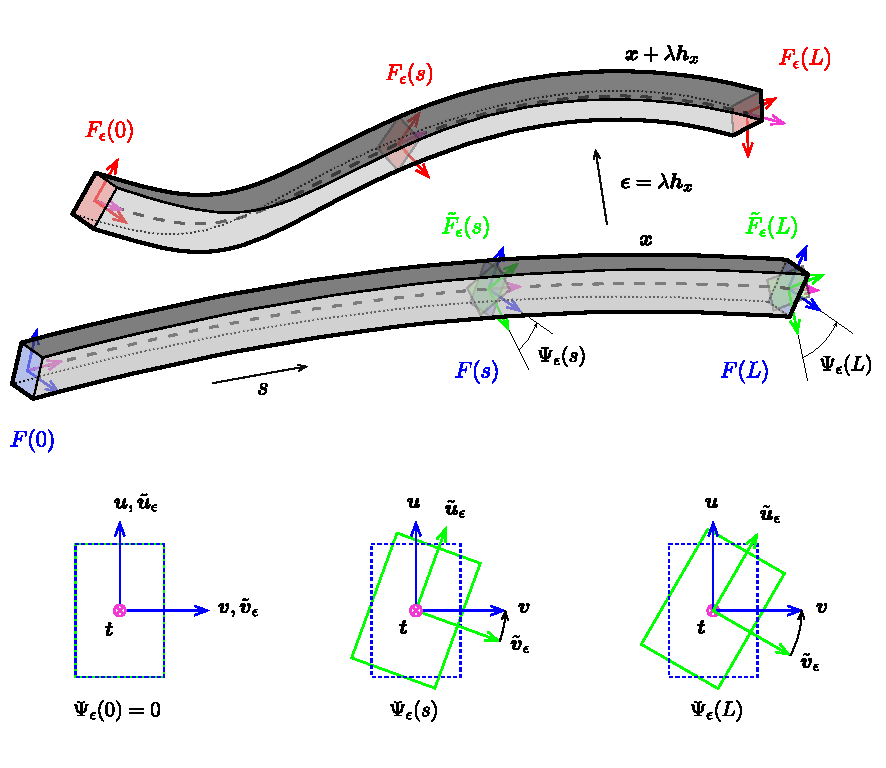
\includegraphics[width=\linewidth]{writhe.pdf}
\caption{Repères de Frenet attachés à  $\gamma$.}
\label{fig:1_1}
\end{figure}

\subsubsection{Calculation of $\Psi_\epsilon$}

\begin{figure}[p]
\centering
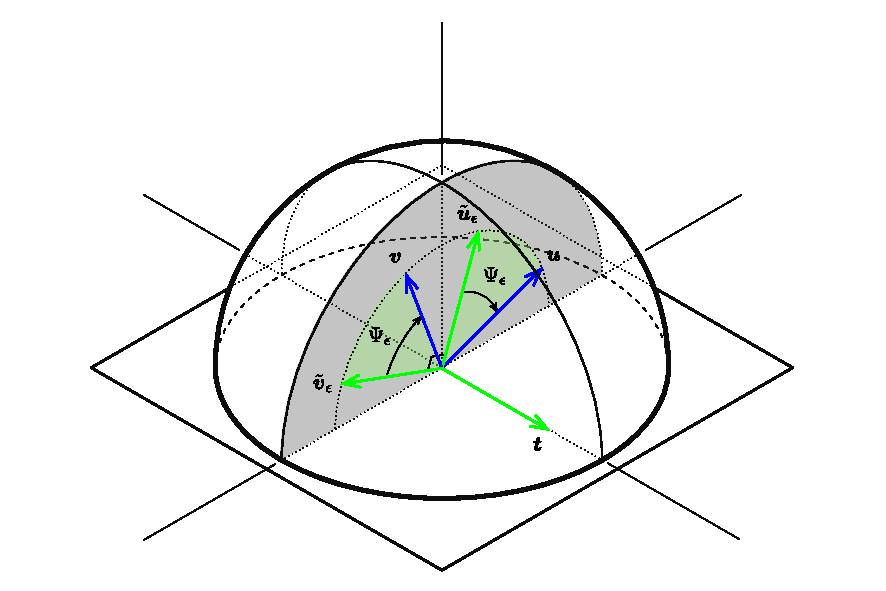
\includegraphics[width=\textwidth]{rotation_A.pdf}
\caption{$F$ is obtained by rotating $\tilde{F}_\epsilon$ around $\vect{t}$ of an angle $\Psi_\epsilon$.}
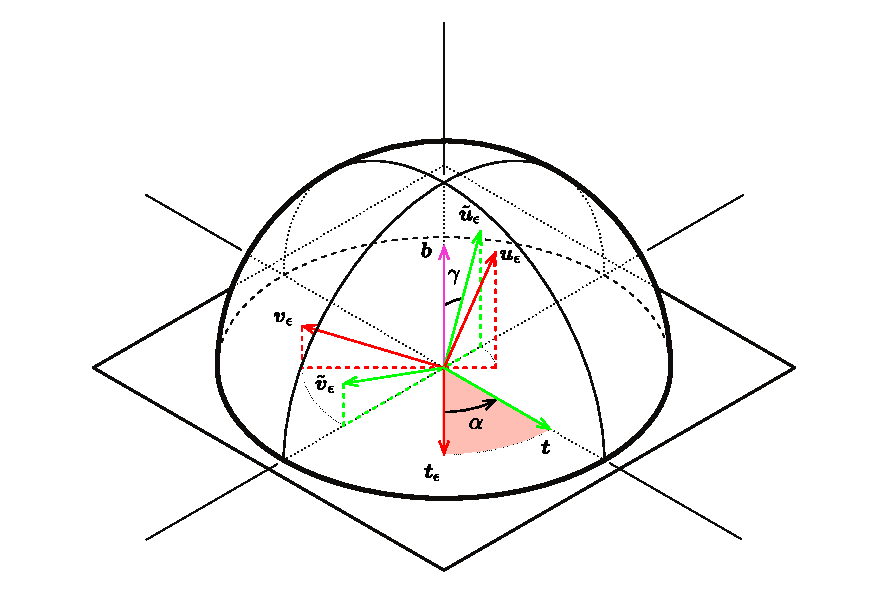
\includegraphics[width=\textwidth]{rotation_B.pdf}
\caption{$\tilde{F}_\epsilon$ is obtained by parallel tranpsporting $F_\epsilon$ from $\vect{t}_\epsilon$ to $\vect{t}$. This operation could be seen as a rotation around $\vect{t}_\epsilon \times \vect{t}$ of an angle $\alpha_\epsilon$.}
\label{A}
\end{figure}

This variation is closely related to the writhe of closed curves. As explained in~\cite{Fuller1978} when parallel transporting an adapted frame around a closed curve it might not realigned with itself after one complete loop. This \guil{lack of alignement} is directly measured by the change of writhe which can be computed with Fuller's Formula~\cite{Fuller1978}.

Note that the derivative of $\theta$ with respect to $\vect{x}$ can be evaluated by the change of writhe in the curve as suggested in~\cite{deVries2005}. This approach is completly equivalent.

One can also see this lack of alignement in terms of rotation. Parallel transport being a propagation of frame from $s = 0$, the cumulated rotation of Bishop frame from the deformed configuration around the initial configuration at arc length $s$ is the cumulated angle of rotation of $\vect{u}[\vect{x} + \lambda\vect{h}_x]$ around $\vect{d}_3[\vect{x}]$. Recalling the rotation rate of $\vect{u}[\vect{x} + \lambda\vect{h}_x]$ is $\vect{\kappa b}[\vect{x} + \lambda\vect{h}_x]$ by definition of zero-twisting frame, one can write~:
\begin{equation}
	\Psi_\epsilon[\vect{x}](s) =
	-\int_0^s \vect{\kappa b}[\vect{x} + \lambda\vect{h}_x] \cdot \vect{d}_3[\vect{x}] \,dt
\end{equation}
The calculation of $\vect{\kappa b}[\vect{x} + \lambda\vect{h}_x]$ is straight forward from the curvature binormal definition~:
\begin{equation}
	\begin{aligned}
	\vect{\kappa b}[\vect{x} + \lambda\vect{h}_x]
	&= (\vect{x} + \lambda\vect{h}_x)' \times (\vect{x} + \lambda\vect{h}_x)'' \\
	&= \vect{\kappa b}[\vect{x}] + \lambda(\vect{x}'\times\vect{h}''_x + \vect{h}'_x\times\vect{x}'') + \lambda^2(\vect{h}'_x \times \vect{h}''_x) \\
	&= \vect{\kappa b}[\vect{x}] + \lambda(\vect{x}'\times\vect{h}''_x + \vect{h}'_x\times\vect{x}'') + o(\lambda)
	\end{aligned}
\end{equation}
Thus, reminding that $\vect{d}_3[\vect{x}] = \vect{x}'$ and $\vect{\kappa b}[\vect{x}]\cdot\vect{d}_3[\vect{x}] = 0$, and using the invariance of circular product by cyclic permutation, one can express~:
\begin{equation}
	\begin{aligned}
		\Psi_\epsilon[\vect{x}](s)
		&= -\int_0^s \vect{\kappa b}[\vect{x} + \lambda\vect{h}_x] \cdot \vect{d}_3[\vect{x}] \,dt\\
		&= - \lambda \int_0^s (\vect{x}'\times\vect{h}''_x + \vect{h}'_x\times\vect{x}'') \cdot \vect{x}' \,dt + o(\lambda)\\
		&= - \lambda \int_0^s \vect{\kappa b}[\vect{x}]\cdot\vect{h}'_x \,dt + o(\lambda)\\
	\end{aligned}
\end{equation}
By integration by parts, dropping the implicit reference to $\vect{x}$ in the notation, and denoting by $\delta_s$ and $H_s$ the Dirac function and the Heaviside step function centered at $s$, $\Psi_\epsilon(s)$ could be rewritten as~:
\begin{equation}
	\begin{aligned}
		\Psi_\epsilon(s)
		&= - \lambda \int_0^s \vect{\kappa b}\cdot\vect{h}'_x \,dt + o(\lambda)\\
		&=  - \lambda \left(\big[\vect{\kappa b} \cdot  \vect{h}_x \big]_0^s - \int_0^s \vect{\kappa b}' \cdot  \vect{h}_x \,dt\right) + o(\lambda)\\
		&= - \lambda \left(\int_0^s \left(\left(\delta_s-\delta_0\right)\vect{\kappa b} - \vect{\kappa b}'\right)\cdot  \vect{h}_x \,dt\right) + o(\lambda)\\
		&= - \lambda \left(\int_0^L \left(\left(\delta_s-\delta_0\right)\vect{\kappa b} - (1-H_s)\vect{\kappa b}'\right)\cdot  \vect{h}_x \,dt\right) + o(\lambda)
	\end{aligned}
\end{equation}
Note that, as expected, $\Psi_\epsilon(s)$ is in first order of $\lambda$ and thus gets negligible when $\lambda$ tends to zero, that is to say when the perturbation of $\vect{x}$ is infinitesimal~:
\begin{equation}
	\lim_{\lambda \to 0} \Psi_\epsilon(s) = 0
\end{equation}

$H_s~: t \mapsto \left\{\begin{array}{c}0  , \quad t<s \\1  , \quad t\geqslant s \end{array}\right.$ est la fonction de Heaviside.

$\delta_s~: t \mapsto \delta(t-s)$ est la distribution de dirac centrée en $s$.

\subsubsection{Calculation of $\alpha_\epsilon$}

Recall that $\tilde{F}_\epsilon$ is obtained by parallel tranpsporting $F_\epsilon$ from $\vect{t}_\epsilon$ to $\vect{t}$.
$\tilde{F}_\epsilon$ results from the rotation of $F_\epsilon$ around $\vect{b} = \vect{t}_\epsilon \times \vect{t}$ by an angle $\alpha_\epsilon$.

Recall from \eqref{eq:3_6} that because the rod is supposed to be unstretchable, $\vect{t}_\epsilon$ stays collinear to $\vect{t}$ for an infinitesimal perturbation of the centerline~:
\begin{equation}
		\|\vect{t}\| = \|\vect{t}_\epsilon\| = 1
		\Rightarrow  (\vect{x}+\vect{\epsilon})' \cdot (\vect{x}+\vect{\epsilon})' = 1
		\Leftrightarrow  \vect{x}'\cdot\vect{\epsilon}' = - \tfrac{\lambda^2}{2}\|\vect{h}_x'\|^2
\end{equation}
Which leeds to~:
\begin{equation}
		\cos \alpha_\epsilon(s) = \vect{t} \cdot \vect{t}_\epsilon = \vect{x}' \cdot (\vect{x}+\vect{\epsilon})'
		= 1 + \vect{x}' \cdot \vect{\epsilon}'
		= 1 - \tfrac{\lambda^2}{2}\|\vect{h}_x'\|^2
\end{equation}

Thus, at second order in $\lambda$~:
\begin{subequations}
	\begin{gather}
		\cos \alpha_\epsilon = 1 - \tfrac{\lambda^2}{2}\|\vect{h}_x'\|^2
		\\
		\sin \alpha_\epsilon = \sqrt{1-\cos^2 \alpha_\epsilon} = \lambda\|\vect{h}_x'\| + o(\lambda^2)
		\\
		\sin^2 {\alpha_\epsilon}{/2} = \tfrac{\lambda^2}{4}\|\vect{h}_x'\|^2
	\end{gather}
\end{subequations}

Finally, it's possible to conclude that $\alpha_\epsilon(s)$ is in first order of $\lambda$ and thus gets negligible when $\lambda$ tends to zero~:
\begin{equation}
	\lim_{\lambda \to 0} \alpha_\epsilon(s) = 0
\end{equation}

%\begin{figure}[t]
%\centering
%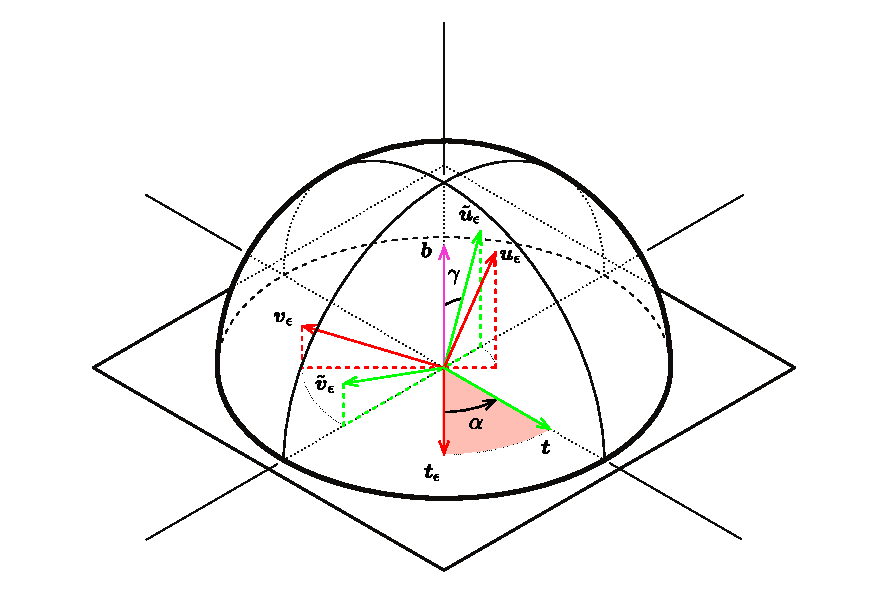
\includegraphics[width=\linewidth]{rotation_B.pdf}
%\caption{$\tilde{F}_\epsilon$ is obtained by parallel tranpsporting $F_\epsilon$ from $\vect{t}_\epsilon$ to $\vect{t}$. This operation could be seen as a rotation around $\vect{t}_\epsilon \times \vect{t}$ of an angle $\alpha$.}
%\label{fig:1_1}
%\end{figure}

\subsubsection{Aligning $\tilde{F}_\epsilon$ towards $F_\epsilon$}
Recall that aligning $\tilde{F}_\epsilon$ over $F$ is nothing but a rotation around $\vect{t}$ by an angle $\Psi_\epsilon$. This leads to~:
\begin{subequations}
%	\left\{
	\begin{gather}
		\vect{\tilde{u}}_\epsilon = \cos{\Psi_\epsilon}\;\vect{u} + \sin{\Psi_\epsilon}\;\vect{v}\\
		\vect{\tilde{v}}_\epsilon = -\sin{\Psi_\epsilon}\;\vect{u} + \cos{\Psi_\epsilon}\;\vect{v}
	\end{gather}
%	\right.
\end{subequations}

\subsubsection{Aligning $F_\epsilon$ towards $\vect{t}$}

Recall that $\tilde{F}_\epsilon$ is obtained by parallel tranpsporting $F_\epsilon$ from $\vect{t}_\epsilon$ to $\vect{t}$. This operation could be seen as a rotation around $\vect{t}_\epsilon \times \vect{t}$ of an angle $\alpha_\epsilon$. Where~:
\begin{equation}
	\vect{b} = \vect{t}_\epsilon \times \vect{t}
	 = \cos{\gamma}\;\vect{\tilde{u}}_\epsilon + \sin{\gamma}\;\vect{\tilde{v}}_\epsilon
	 = \cos{\gamma}\;\vect{u}_\epsilon + \sin{\gamma}\;\vect{v}_\epsilon
\end{equation}
Expressing $F_\epsilon$ on the basis $\tilde{F}_\epsilon$ gives for $\vect{u}_\epsilon$ and $\vect{v}_\epsilon$~:
\begin{subequations}
\begin{gather}
		\vect{u}_\epsilon = \sin{\gamma}\;\vect{b} + \cos{\gamma}\;\big(\sin{\alpha_\epsilon}\;\vect{\tilde{t}}
	+ \cos{\alpha_\epsilon}\;(\cos{\gamma}\;\vect{\tilde{u}_\epsilon}
	- \sin{\gamma}\;\vect{\tilde{v}_\epsilon})\big)
		\\
		\vect{v}_\epsilon = \cos{\gamma}\;\vect{b} + \sin{\gamma}\;\big(-\sin{\alpha_\epsilon}\;\vect{\tilde{t}}
	+ \cos{\alpha_\epsilon}\;(\sin{\gamma}\;\vect{\tilde{u}_\epsilon}
	- \cos{\gamma}\;\vect{\tilde{v}_\epsilon})\big)
\end{gather}
\end{subequations}
Which can be rearranged in~:
\begin{subequations}
\begin{gather}
		\vect{u}_\epsilon = \cos{\gamma}\sin{\alpha_\epsilon}\;\vect{t}
	+ (\cos{\alpha_\epsilon}\cos^2{\gamma}+ \cos^2{\gamma})\vect{\tilde{u}_\epsilon}
	+ \sin{\gamma}\cos{\gamma}\;(1-\cos{\alpha_\epsilon})\vect{\tilde{v}_\epsilon}
		\\
		\vect{v}_\epsilon = -\sin{\gamma}\sin{\alpha_\epsilon}\;\vect{t}
	+ \cos{\gamma}\sin{\gamma}\;(1-\cos{\alpha_\epsilon})\vect{\tilde{u}_\epsilon}
	+ (\cos^2{\gamma} + \cos{\alpha_\epsilon}\sin^2{\gamma})\vect{\tilde{v}_\epsilon}
\end{gather}
\end{subequations}

\subsubsection{Variation of Bishop frame with respect to $x$}
Finally, one can express $F_\epsilon$ on the basis $F$ as the composition of two rotations~:
\begin{subequations}
	\begin{gather}
	\vect{u}_\epsilon =
	\begin{bmatrix}
		1 & 0 & 0 \\
		0 & \cos{\Psi_\epsilon} & -\sin{\Psi_\epsilon} \\
		0 & \sin{\Psi_\epsilon} & \cos{\Psi_\epsilon}
	\end{bmatrix}
	\begin{bmatrix}
		\cos{\gamma}\sin{\alpha_\epsilon} \\
		1-2\cos^2{\gamma}\sin^2{\alpha_\epsilon/2} \\
		2\sin{\gamma}\cos{\gamma}\sin^2{\alpha_\epsilon/2}
	\end{bmatrix}
	=
	\begin{bmatrix}
		\alpha_\epsilon\cos{\gamma}\\
		1 \\
		\Psi_\epsilon
	\end{bmatrix}
	+ o(\lambda)
	\\
	\vect{v}_\epsilon =
	\begin{bmatrix}
		1 & 0 & 0 \\
		0 & \cos{\Psi_\epsilon} & -\sin{\Psi_\epsilon} \\
		0 & \sin{\Psi_\epsilon} & \cos{\Psi_\epsilon}
	\end{bmatrix}
	\begin{bmatrix}
		-\sin{\gamma}\sin{\alpha_\epsilon} \\
		2\sin{\gamma}\cos{\gamma}\sin^2{\alpha_\epsilon/2} \\
		1-2\sin{\gamma}^2\sin^2{\alpha_\epsilon/2}
	\end{bmatrix}
	=
	\begin{bmatrix}
		-\alpha_\epsilon\sin{\gamma}\\
		-\Psi_\epsilon \\
		1
	\end{bmatrix}
	+ o(\lambda)
	\end{gather}
\end{subequations}

%\begin{equation}
%
%\end{equation}
Here, the expressions have been developed in first order of $\lambda$ as far as $\alpha_\epsilon$ and $\Psi_\epsilon$ it's been proofed in eq [] that those quantities tends two zero when the perturbation of the centerline is infinitesimal.

Finally, one can express the variation of material directors with respect to an infinitesimal variation of rod's centerline~:
\begin{subequations}
\begin{gather}
		\vect{u}_\epsilon = \alpha_\epsilon\cos{\gamma}\;\vect{t} + \vect{u} + \Psi_\epsilon\vect{v} + o(\lambda)
		\\
		\vect{v}_\epsilon = -\alpha_\epsilon\sin{\gamma}\;\vect{t} + \vect{v} - \Psi_\epsilon\vect{u} + o(\lambda)
\end{gather}
\end{subequations}

\subsubsection{Variation of material frame with respect to $\vect{x}$}
Recalling the expression of the material frame expressed in the reference Bishop frame, it's now easy to deduce the variation of material frame with respect to a variation of the rod's centerline~:
\begin{subequations}
		\begin{gather}
			\vect{d}_1[\vect{x}+\lambda \vect{h}_x] =
			\cos{\theta} \; \vect{u}_\epsilon + \sin{\theta} \; \vect{v}_\epsilon\\
			\vect{d}_2[\vect{x}+\lambda \vect{h}_x] =
			-\sin{\theta} \; \vect{u}_\epsilon + \cos{\theta} \; \vect{v}_\epsilon
		\end{gather}
\end{subequations}
Which leads according to the previous equation to~:
\begin{subequations}
	\begin{gather}
		\vect{d}_1[\vect{x}+\lambda \vect{h}_x] = \vect{d}_1[\vect{x}] + \Psi_\epsilon\vect{d}_2[\vect{x}] + \alpha_\epsilon\cos{(\theta-\gamma)}\;\vect{t}[\vect{x}] + o(\lambda) \\
		\vect{d}_2[\vect{x}+\lambda \vect{h}_x] = \vect{d}_2[\vect{x}] - \Psi_\epsilon\vect{d}_1[\vect{x}] - \alpha_\epsilon\sin{(\theta+\gamma)}\;\vect{t}[\vect{x}] + o(\lambda)
		\end{gather}
\end{subequations}

\subsection{Derivative of the material curvatures vector with respect to $x$}

It's know straightforward from the previous section to express the variation of the material curvatures with respect to a variation $\vect{\epsilon} =\lambda \vect{h}_x$ of $\vect{x}$ while $\theta$ remains unchanged.
\begin{subequations}
	\begin{gather}
		(\vect{x}+\lambda \vect{h}_x)'' \cdot \vect{d}_1[\vect{x}+\lambda \vect{h}_x] =
			(\vect{x}''+\lambda \vect{h}_x'')\cdot\big(\vect{d}_1 + \Psi_\epsilon\vect{d}_2
			+ \alpha_\epsilon\cos{(\theta-\gamma)}\;\vect{t} + o(\lambda)\big) \\
		(\vect{x}+\lambda \vect{h}_x)'' \cdot \vect{d}_2[\vect{x}+\lambda \vect{h}_x] =
			(\vect{x}''+\lambda \vect{h}_x'')\cdot\big(\vect{d}_2 - \Psi_\epsilon\vect{d}_1
			- \alpha_\epsilon\sin{(\theta+\gamma)}\;\vect{t} + o(\lambda)\big)
		\end{gather}
\end{subequations}
Thus, recalling that $\vect{x}''\cdot\vect{d}_3 = 0$ and that $\alpha_\epsilon$ and $\Psi_\epsilon$ are first order quantities in $\lambda$~:
\begin{subequations}
	\begin{gather}
		(\vect{x}+\lambda \vect{h}_x)'' \cdot \vect{d}_1[\vect{x}+\lambda \vect{h}_x] = 					\vect{x}''\cdot\vect{d}_1 + \Psi_\epsilon\vect{x}''\cdot\vect{d}_2 + \lambda \vect{h}_x''\cdot\vect{d}_1 + o(\lambda)\\
		(\vect{x}+\lambda \vect{h}_x)'' \cdot \vect{d}_2[\vect{x}+\lambda \vect{h}_x] =
				\vect{x}''\cdot\vect{d}_2 - \Psi_\epsilon\vect{x}''\cdot\vect{d}_1 +  \lambda \vect{h}_x''\cdot\vect{d}_2 + o(\lambda)
	\end{gather}
\end{subequations}
Which finally leads to~:
\begin{equation}
		\vect{\omega}[\vect{x}+\lambda \vect{h}_x]  =
		\vect{\omega}[\vect{x}] - \Psi_\epsilon\mat{J}\vect{\omega}[\vect{x}]+\lambda
		\begin{bmatrix}
			-\vect{h}_x''\cdot\vect{d}_2\\
			\vect{h}_x''\cdot\vect{d}_1\\
		\end{bmatrix} + o(\lambda)
\end{equation}
Reminding the expression of $\Psi_\epsilon$ computed in paragraphe[], one can express the derivative of the material curvatures vector with respect to $\vect{x}$~:
\begin{equation}
			\pdiffof{x}{\vect{\omega}}{s}{\vect{h}_x}
	= 	\left(\int_0^L \left(\left(\delta_s-\delta_0\right)\vect{\kappa b} - (1-H_s)\vect{\kappa b}'\right)\cdot  \vect{h}_x \,dt\right)\mat{J}\vect{\omega}+
		\begin{bmatrix}
			-{\vect{d}_2}^T\\
			{\vect{d}_1}^T\\
		\end{bmatrix}\cdot \vect{h}_x''
\end{equation}


\subsection{Computation of the forces acting on the centerline}

The forces acting on the centerline are given by the functional derivative of the potential elastic energy with respect to $x$ which can be decomposed according to the chaine rule~:
\begin{equation}
	\begin{aligned}
	\scalar{-f(s)}{\vect{h}_x} = \pdiffof{x}{\mathcal{E}}{s}{\vect{h}_x}
	&= \pdiffof{x}{\mathcal{E}_b}{s}{\vect{h}_x} + \pdiffof{x}{\mathcal{E}_t}{s}{\vect{h}_x} \\
	&= \pdiffof{x}{\mathcal{E}_b[\vect{\omega}[\vect{x}]]}{s}{\vect{h}_x} + \pdiffof{x}{\mathcal{E}_t[\vect{x}]}{s}{\vect{h}_x} \\
	\end{aligned}
\end{equation}

\subsubsection{Derivative of the torsion energy with respect to $x$}

Recall that the torsion energy only depends on $\theta$ which is independent of $x$. Thus, $\mathcal{E}_t$ is independent of $x$~:
\begin{equation}
	\pdiffof{x}{\mathcal{E}_t[\vect{x}]}{s}{\vect{h}_x}
		= \frac{d}{d\lambda} \mathcal{E}_t[\vect{x} + \lambda \vect{h}_x]\Bigr|_{\lambda = 0} = 0
\end{equation}

\subsubsection{Derivative of the bending energy with respect to $x$}

The derivative of $\mathcal{E}_b$ is obtained with the chaine rule~:
\begin{equation}
	\pdiffof{\omega}{\mathcal{E}_b[\vect{\omega}]}{s}{\vect{h}_\omega}
		= \frac{d}{d\lambda} \mathcal{E}_b[\vect{\omega} + \lambda \vect{h}_\omega]\Bigr|_{\lambda = 0}
		= \int_{0}^{L} (\vect{\omega} - \rconf{\vect{\omega}})^T \mat{B} \cdot \vect{h}_\omega \;dt
\end{equation}
Finally, reminding eq 4.14~:
\begin{equation}
	\pdiffof{x}{\mathcal{E}_b[\vect{\omega}[\vect{x}]]}{s}{\vect{h}_x}
	= \pdiffof{\omega}{\mathcal{E}_b[\vect{\omega}]}{s}{(\pdiffof{x}{\vect{\omega}[\vect{x}]}{s}{\vect{h}_x})}
	= \mathcal{A} +\mathcal{B}+\mathcal{C}
\end{equation}
Where~:
\begin{subequations}
	\begin{gather}
	\mathcal{A} = \int_{0}^{L} (\vect{\omega} - \rconf{\vect{\omega}})^T \mat{B}
	\begin{bmatrix}
		-{\vect{d}_2}^T\\
		{\vect{d}_1}^T\\
	\end{bmatrix}\cdot \vect{h}_x'' \;dt \\
	\mathcal{B} =
	\int_{t=0}^{L} (\vect{\omega} - \rconf{\vect{\omega}})^T \mat{B}\mat{J}\vect{\omega}
	\left(\int_{u=0}^L \left(\delta_t-\delta_0\right)\vect{\kappa b}\cdot  \vect{h}_x \;du\right)
	\;dt\\
	\mathcal{C} =
	\int_{t=0}^{L} -(\vect{\omega} - \rconf{\vect{\omega}})^T \mat{B}\mat{J}\vect{\omega}
	\left(\int_{u=0}^L \left(1-H_t\right)\vect{\kappa b}'\cdot  \vect{h}_x \;du\right)
	\;dt
	\end{gather}
\end{subequations}

Calculus of $\mathcal{A}$~:
\begin{equation}
	\mathcal{A}
	= \int_{0}^{L} (\vect{\omega} - \rconf{\vect{\omega}})^T \mat{B}
		\begin{bmatrix}
			-{\vect{d}_2}^T\\
			{\vect{d}_1}^T\\
		\end{bmatrix}\cdot \vect{h}_x'' \;dt \\
\end{equation}

Recalling the bending moment is given by~:
\begin{equation}
	\vect{M}
	= (\kappa_1 - \rconf{\kappa}_1)EI_1\vect{d}_1 + (\kappa_2 - \rconf{\kappa}_2)EI_2\vect{d}_2
	= M_1\vect{d}_1 + M_2\vect{d}_2
\end{equation}
One can remark that~:
\begin{equation}
	\left(\vect{\omega} - \rconf{\vect{\omega}}\right)^T \mat{B}
		\begin{bmatrix}
			-{\vect{d}_2}^T\\
			{\vect{d}_1}^T\\
		\end{bmatrix}
	=  M_2{\vect{d}_1}^T - M_1{\vect{d}_2}^T
	= - ({\vect{d}_3} \times \vect{M})^T
\end{equation}

\note{
Rq~: on mixe abusivement 2 formes d'écritures, matricielle et vectorielle, à cause du produit scalaire que l'on écrit tantôt sous sa forme vectorielle et parfois matricielle (à l'aide de la transposée).}

Thus,  $\mathcal{A}$ could be rewritten in it's vectoriel form~:
\begin{equation}
	\begin{aligned}
	\mathcal{A}
	& = -\int_{0}^{L} ({\vect{d}_3} \times \vect{M}) \cdot \vect{h}_x'' \;dt \\
	& = -\left[\left({\vect{d}_3} \times \vect{M}\right) \cdot \vect{h}_x'\right]_0^L
		+ \int_{0}^{L} \left({\vect{d}_3} \times \vect{M}\right)'\cdot \vect{h}_x' \;dt \\
	& = -\left[\left({\vect{d}_3} \times \vect{M}\right) \cdot \vect{h}_x'\right]_0^L
		+ \int_{0}^{L} \left(
			\left({\vect{d}_3} \times \vect{M}'\right) \cdot \vect{h}_x'
			+ \left({\vect{h}'_x} \times \vect{d}_3'\right) \cdot \vect{M}
			 \right)\;dt \\
	\end{aligned}
\end{equation}
Recall that from \eqref{eq:3_6} that $\vect{h}'_x \cdot \vect{d}_3 = 0$  and from \eqref{eq:3_1} that $\vect{d}'_3 \cdot \vect{d}_3 = 0$. Hence, $\vect{h}'_x \times \vect{d}_3'$ is colinear to $\vect{d}_3$. Or by definition $\vect{M}$ is orthogonal to $\vect{d}_3$. Thus, $\left({\vect{h}'_x} \times \vect{d}_3'\right) \cdot \vect{M} = 0$.
Finally, after a second integration by parts~:
\begin{equation}
	\begin{aligned}
	\mathcal{A}
	& = -\left[\left({\vect{d}_3} \times \vect{M}\right) \cdot \vect{h}_x'\right]_0^L
		+ \int_{0}^{L} \left(
			{\vect{d}_3} \times \vect{M}'\right) \cdot \vect{h}_x'
			 \;dt \\
	& = 	\left[
			({\vect{d}_3} \times \vect{M}') \cdot \vect{h}''_x\
			- ({\vect{d}_3} \times \vect{M}) \cdot \vect{h}_x'
		\right]_0^L
		- \int_{0}^{L} \left({\vect{d}_3} \times \vect{M}'\right)' \cdot \vect{h}_x \;dt \\
	\end{aligned}
\end{equation}

Calculus of $\mathcal{B}$~:
\begin{equation}
	\begin{aligned}
	\mathcal{B} &=
	\int_{t=0}^{L} (\vect{\omega} - \rconf{\vect{\omega}})^T \mat{B}\mat{J}\vect{\omega}
	\left(\int_{u=0}^L \left(\delta_t-\delta_0\right)\vect{\kappa b}\cdot  \vect{h}_x \,du\right)
	\;dt
	\\
	&=
	-\left(\vect{\kappa b}\cdot\vect{h}_x\right)(0) \int_{t=0}^{L} (\vect{\omega} - \rconf{\vect{\omega}})^T \mat{B}\mat{J}\vect{\omega}\;dt
	+
	\int_{t=0}^{L} (\vect{\omega} - \rconf{\vect{\omega}})^T \mat{B}\mat{J}\vect{\omega}
	\vect{\kappa b}\cdot\vect{h}_x
	\;dt
	\end{aligned}
\end{equation}

Calculus of $\mathcal{C}$~:
\begin{equation}
	\begin{aligned}
	\mathcal{C} &=
	\int_{t=0}^{L} -(\vect{\omega} - \rconf{\vect{\omega}})^T \mat{B}\mat{J}\vect{\omega}
	\left(\int_{u=0}^L \left(1-H_t\right)\vect{\kappa b}'\cdot  \vect{h}_x \;du\right)
	\;dt
	\\
	&=
	\int_{u=0}^{L}\int_{t=u}^{L}-\left((\vect{\omega} - \rconf{\vect{\omega}})^T \mat{B}\mat{J}\vect{\omega}\right)(t)
	\left(\vect{\kappa b}'\cdot \vect{h}_x\right)(u) \;dt\;du
	\\
	&=
	\int_{u=0}^{L}-\left(\int_{t=u}^{L}(\vect{\omega} - \rconf{\vect{\omega}})^T \mat{B}\mat{J}\vect{\omega}\;dt\right)
	\left(\vect{\kappa b}'\cdot \vect{h}_x\right)\;du
	\\
	\end{aligned}
\end{equation}
By several integration by parts, using Fubini's theorem once and supposing that the terms vanishes at $s=0$ and $s=L$~:
\begin{equation}
	\begin{aligned}
	\mathcal{B}+\mathcal{C} &=
	\int_{t=0}^{L} \left(
	(\vect{\omega} - \rconf{\vect{\omega}})^T \mat{B}\mat{J}\vect{\omega}
	\vect{\kappa b}
	-
	\left(\int_{u=t}^{L}(\vect{\omega} - \rconf{\vect{\omega}})^T \mat{B}\mat{J}\vect{\omega}\;du\right)
	\vect{\kappa b}'
	\right)\cdot \vect{h}_x \;dt\\
	&=
	\int_{t=0}^{L} \left(
	-\left(\int_{u=t}^{L}(\vect{\omega} - \rconf{\vect{\omega}})^T \mat{B}\mat{J}\vect{\omega}\;du\right)'
	\vect{\kappa b}
	-
	\left(\int_{u=t}^{L}(\vect{\omega} - \rconf{\vect{\omega}})^T \mat{B}\mat{J}\vect{\omega}\;du\right)
	\vect{\kappa b}'
	\right)\cdot \vect{h}_x \;dt\\
	&=
	\int_{t=0}^{L} \left(
	-\left(\int_{u=t}^{L}(\vect{\omega} - \rconf{\vect{\omega}})^T \mat{B}\mat{J}\vect{\omega}\;du\right)
	\vect{\kappa b}
	\right)'\cdot \vect{h}_x \;dt\\
	\end{aligned}
\end{equation}

Which can be rewritted using the quasi-static hypothesis~:
\begin{equation}
	\begin{aligned}
	\mathcal{B}+\mathcal{C}
	&=
	\int_{t=0}^{L} \left(
	-\left(\int_{u=t}^{L}(\vect{\omega} - \rconf{\vect{\omega}})^T \mat{B}\mat{J}\vect{\omega}\;du\right)
	\vect{\kappa b}
	\right)'\cdot \vect{h}_x \;dt\\
	&=
	\int_{t=0}^{L} \left(
	-\left(
	\int_{u=t}^{L}\beta(\theta' -{\rconf{\theta}'})(\delta_L-\delta_0) - \left(\beta(\theta' -{\rconf{\theta}'})\right)'\;du
	\right)
	\vect{\kappa b}
	\right)'\cdot \vect{h}_x \;dt\\
	&=
	\int_{t=0}^{L} \left(
	-\left(
	\beta(\theta' -{\rconf{\theta}'})(L) - \left[\beta(\theta' -{\rconf{\theta}'})\right]_t^L
	\right)
	\vect{\kappa b}
	\right)'\cdot \vect{h}_x \;dt\\
		&=
	\int_{t=0}^{L} -\left(
	\beta(\theta' -{\rconf{\theta}'})
	\vect{\kappa b}
	\right)'\cdot \vect{h}_x \;dt\\
	\end{aligned}
\end{equation}

Finally~:
\begin{equation}
		\pdiffof{x}{\mathcal{E}_b[\vect{\omega}[\vect{x}]]}{s}{\vect{h}_x}
		=
		\int_{0}^{L} \left(
		- \left({\vect{d}_3} \times \vect{M}'\right)'
		- \left(\beta(\theta' -{\rconf{\theta}'}) \vect{\kappa b}\right)'
		\right)\cdot \vect{h}_x \;dt\\
\end{equation}

\subsubsection{Internal forces}

Thus, the internal forces are related to the variation of internal elastic energy as~:
\begin{equation}
	\begin{aligned}
	\scalar{-\vect{f}(s)}{\vect{h}_x} &= \pdiffof{x}{\mathcal{E}}{s}{\vect{h}_x}
		=
		- \int_{0}^{L} \left(
		\left({\vect{d}_3} \times \vect{M}'\right)'
		+ \left(\beta(\theta' -{\rconf{\theta}'}) \vect{\kappa b}\right)'
		\right)\cdot \vect{h}_x \;dt\\
	\end{aligned}
\end{equation}
Finally, we can conclude on the expression of the internal forces~:
\begin{equation}
	\vect{f}(s) = \left({\vect{d}_3} \times \vect{M}'\right)'
		+ \left(\beta(\theta' -{\rconf{\theta}'}) \vect{\kappa b}\right)'
\end{equation}


\note{
Remarquer ici que l'expression est purement locale.
Elle ne dépend pas du sens de parcours de la poutre, contrairement au raisonnement suivi.
Cette différence est notable avec la démarche de B. Audoly.
Faire le bilan des bénéfices de l'hypothèse quasi-statique~:
- expressions rigoureusement vraies à  l'équilibre statique
- simplification ds le calcul des efforts
- rapidité dans le calcul avec des expressions plus simples
- il n'est pas forcément intéressant en terme d'algorithmie d'imposer l'hypothèse quasistatique au cours du calcul. Il faudrait faire un bench pour savoir.

On retombe sur les équations de Kirchhoff à un terme manquant pret. Qui exprime la contribution de la variation moment de flexion à cause de la torsion $\tau \vect{M}`$. Peut-être que ce terme est finalement d'un ordre supérieur, si l'on suppose une variation lente de la torsion ? Comment comprendre la disparition de ce terme qui semble nécessaire à l'équilibre statique d'un élément de poutre si l'on en croit les équations de Kirchhoff ?

}

\section{Conclusion}

On retrouve les équations de kirchhoff dynamique où l'on a négligé les forces inertielles de rotation d'un élément de poutre autour de $\vect{d}_1$ et $\vect{d}_2$ pour ne garder que la dynamique de rotation de la section autour de la fibre neutre $\vect{d}_3$.

The shear force acting on the right side of a section is nothing but $\vect{T} = \int \vect{f}$~:
\begin{equation}
	\vect{T}(s) = \vect{d}_3 \times \vect{M}'
		+ Q \vect{\kappa b}
\end{equation}
The linear momentum acting on the centerline is given by~:
\begin{equation}
	m(s) = Q' - \vect{\kappa b} \cdot (\vect{d}_3 \times \mat{M})
\end{equation}
 The main hypothesis are~:
\begin{itemize}
\item Bernoulli~: $\vect{d}_i \cdot \vect{d}_j = \delta_{ij}$
\item Inextensibility~: $\|\vect{d}'_3\| = 1$
\item Quasistatic~: at each timestep regarding bending motion $m(s) = 0$
\end{itemize}

